\section*{Introduction}\label{introduction}
\addcontentsline{toc}{section}{Introduction}

Until the end of the 90s, Plan-Space Planning (PSP) was generally
preferred by the automated planning community. Its early commitment,
expressiveness, and flexibility were clear advantages over State-Space
Planning (SSP). However, more recently, drastic improvements in state
search planning were made possible by advanced and efficient heuristics.
This allowed those planners to scale up more efficiently than plan-space
search ones, notably thanks to approaches like GraphPlan
{[}\protect\hyperlink{ref-blumux5ffastux5f1997}{1}{]}, fast-forward
{[}\protect\hyperlink{ref-hoffmannux5fffux5f2001}{2}{]}, LAMA
{[}\protect\hyperlink{ref-richterux5flamaux5f2011}{3}{]} and Fast
Downward Stone Soup
{[}\protect\hyperlink{ref-rogerux5ffastux5f2014}{4}{]}. This evolution
led to a preference for performances upon other aspects of the problem
of automated planning. However, some of these aspects can be more easily
addressed in Partial Order Planning (POP), also known as Partial Order
Causal Link (POCL) planning. For example POP, can take advantage of
least commitment
{[}\protect\hyperlink{ref-mccluskeyux5fengineeringux5f1997}{5}{]} that
offers more flexibility with a partial plan that describes only the
necessary order of the actions and not a fixed sequence of steps. POP
has been proven to be well suited for multi-agent planning
{[}\protect\hyperlink{ref-kvarnstromux5fplanningux5f2011}{6}{]} and
temporal planning
{[}\protect\hyperlink{ref-bentonux5ftemporalux5f2012}{7}{]} . These
advantages made UCPOP
{[}\protect\hyperlink{ref-penberthyux5fucpopux5f1992}{8}{]} one of the
preferred POP planners of its time with works made to port some of its
characteristics into state-based planning
{[}\protect\hyperlink{ref-gazenux5fcombiningux5f1997}{9}{]}.

Related works already tried to explore new ideas to make POP an
attractive alternative to regular state-based planners like the
appropriately named ``Reviving partial order planning''
{[}\protect\hyperlink{ref-nguyenux5frevivingux5f2001}{10}{]} and VHPOP
{[}\protect\hyperlink{ref-younesux5fvhpopux5f2003}{11}{]}. More recent
efforts
{[}\protect\hyperlink{ref-colesux5fforwardchainingux5f2010}{12}{]},
{[}\protect\hyperlink{ref-sapenaux5fcombiningux5f2014}{13}{]} are trying
to adapt the powerful heuristics from state-based planning to POP's
approach. An interesting approach of these last efforts is found in
{[}\protect\hyperlink{ref-shekharux5flearningux5f2016}{14}{]} with
meta-heuristics based on offline training on the domain. However, we
clearly note that only a few papers lay the emphasis upon plan quality
using POP {[}\protect\hyperlink{ref-ambiteux5fplanningux5f1997}{15}{]},
{[}\protect\hyperlink{ref-estlinux5flearningux5f1997}{16}{]}.

The present paper lays the base for our project for an intelligent
robotic system that aims to use inverted planning for plan inference in
order to help dependent persons to accomplish tasks. This project is
based on the works of Ramirez et al.
{[}\protect\hyperlink{ref-ramirezux5fplanux5f2009}{17}{]} on inverted
planning for plan inference. This context led us to seek ways to improve
POP with better refining techniques and resolver selection. Since we
need to handle data derived from limited robotic sensors, we need a way
for the planner to be able to be resilient to misleading input plans.
Another aspect of this work lies in the fact that the final system will
need to compute online planning with a feed of observational data. In
order to achieve this we need a planner that can:

\begin{itemize}
\tightlist
\item
  repair and optimize existing plans,
\item
  perform online planning efficiently
\item
  retain performances on complex but medium sized problems.
\end{itemize}

Classical POP algorithms don't meet most of these criteria but can be
enhanced to fit the first one. Usually, POP algorithms take a problem as
an input and use a loop or a recursive function to refine the plan into
a solution. We can't simply use the refining recursive function in order
to be able to use our existing partial plan. This causes multiples side
effects if the input plan is suboptimal. \emph{Our view} on the problem
diverges from other works: PSP is a very different approach compared to
SSP. It is usually more computationally expensive than modern state
space planners but brings several advantages. We want to make the most
of them instead of trying to change POP's fundamental nature. That view
is at the core of our model: we use the refining and least commitment
abilities of POP in order to improve online performances and quality. In
order to achieve this, we start by computing a \emph{proper plan} that
is computed offline with the input of the domain. The explanation of the
way this notion is defined and used is given in \cref{sec:properplan} of
the present paper. Using existing partial plans as input leads to
several issues, mainly with new flaw types that aren't treated in
classical POP. This is why we focus the \cref{sec:negative} of our paper
on plan quality and negative refinements. We, therefore, introduce new
negative flaws and resolvers that aim to fix and optimize the plan: the
\emph{alternative} and the \emph{orphan} flaws. Side effects of negative
flaws and resolvers can lead to conflicts. In order to avoid them and
enhance performances and quality, the algorithm needs resolver and flaw
selection mechanisms that are explained in the \cref{sec:selection}. All
these mechanisms are part of our aLternative Optimization with partiaL
pLan Injection Partial Ordered Planning (LOLLIPOP) algorithm presented
in details in \cref{sec:algorithm}. We prove that the use of these new
mechanisms keeps LOLLIPOP sound and complete in \cref{sec:analysis}.
Experimental results and benchmarks are presented and explained in the
\cref{sec:results} of this paper.

\section{Partial Order Planning
Preliminaries}\label{partial-order-planning-preliminaries}

\subsection{Notation}\label{notation}

For the rest of this paper, we will use the notation defined in
\cref{tbl:symbols}. In order to make some writings more concise, we use
the symbol \(\pm\) to signify that there is a notation for the positive
and negative symbols but the current formula works regardless the sign.
All related notions will be defined later.

\begin{table}\footnotesize
\centering

\caption{\label{tbl:symbols}Most used symbols in the paper. }

\begin{tabular}{@{}ll@{}}
\toprule

Symbol & Description \\\midrule

\(pre(o)\), \(eff(o)\) & Preconditions and effects of the operator
\(o\) \\
\(\Delta\) & Planning domain \\
\(\Pi\) & Planning problem \\
\(T.x\) & Access element \(x\) of tuple \(T\) \\
\(l_{\rightarrow}\), \(l_{\leftarrow}\) & Source and target of the
causal link \(l\) \\
\(o_1 \succ o_2\) & Precedence operator (\(o_1\) precedes \(o_2\)) \\
\(O^P\) & Proper plan of the set of operators \(O\) \\
\(p.d^\pm(o)\) & Outgoing and incoming degrees of \(o\) \\
\(o.d^\pm\) & Proper degrees of \(o\) (\(|pre(o)|\) and \(|eff(o)|\)) \\
\(p.L^\pm(o)\) & Outgoing and incoming causal links of \(o\) \\
\(C(p)\) & Set of cycles in partial plan \(p\) \\
\(C_p(o)\) & Set of cycles in \(p\), \(o\) is part of \\
\(SC_p(o)\) & \(\{o\}\) if \(o\) has a self cycle in \(p\),
\(\emptyset\) otherwise \\
\(F^\pm(p)\) & Set of flaws in \(p\) \\
\(r(f)\) & Resolvers of the flaw \(f\) \\
\(f.n\) & Needer of the flaw \(f\) \\
\(f(p)\) & Application of the flaw \(f\) on plan \(p\) \\
\(fs(p)\) & Full support of \(p\) \\
\(p \models \Pi\) & The partial plan \(p\) is a valid solution of
\(\Pi\) \\

\bottomrule
\end{tabular}

\end{table}

\subsection{Basic Definitions}\label{basic-definitions}

Planning systems need a representation of its fluents and operators. Our
framework is based on a classical domain definition. This is defined in
the following definition from
{[}\protect\hyperlink{ref-gobelbeckerux5fcomingux5f2010}{18}{]}.

\begin{definition}[Domain]\label{def:domain}

We define our planning domain as a tuple
\(\Delta = \langle T, C, P, F, O \rangle\) where

\begin{itemize}
\tightlist
\item
  \(T\) are the \textbf{types},
\item
  \(C\) is the set of \textbf{domain constants},
\item
  \(P\) is the set of \textbf{properties} with their arities and typing
  signatures,
\item
  \(F\) represents the set of \textbf{fluents} defined as potential
  equations over the terms of the domain,
\item
  \(O\) is the set of optionally parameterized \textbf{operators} with
  preconditions and effects.
\end{itemize}

\end{definition}

Along with a domain, every planner needs a problem representation. For
this, we use the classical problem representation with some special
additions.

\begin{definition}[Problem]\label{def:problem}

The planning problem is defined as a tuple
\(\Pi = \langle \Delta, C_\Pi, I, G, p\rangle\) where

\begin{itemize}
\tightlist
\item
  \(\Delta\) is a planning domain,
\item
  \(C_\Pi\) is the set of \textbf{problem constants} disjoint from the
  domain constraints \(C\),
\item
  \(I\) is the \textbf{initial state},
\item
  \(G\) is the \textbf{goal},
\item
  \(p\) is a given \textbf{partial plan}.
\end{itemize}

\end{definition}

The framework uses the \emph{closed world assumption} in which all
predicates and properties that aren't defined in the initial step are
assumed false or don't have a value.

\Cref{fig:example} portrays an example of a planning domain and problem
that we use as a guideline throughout the article.

\begin{figure}[htbp]
\centering
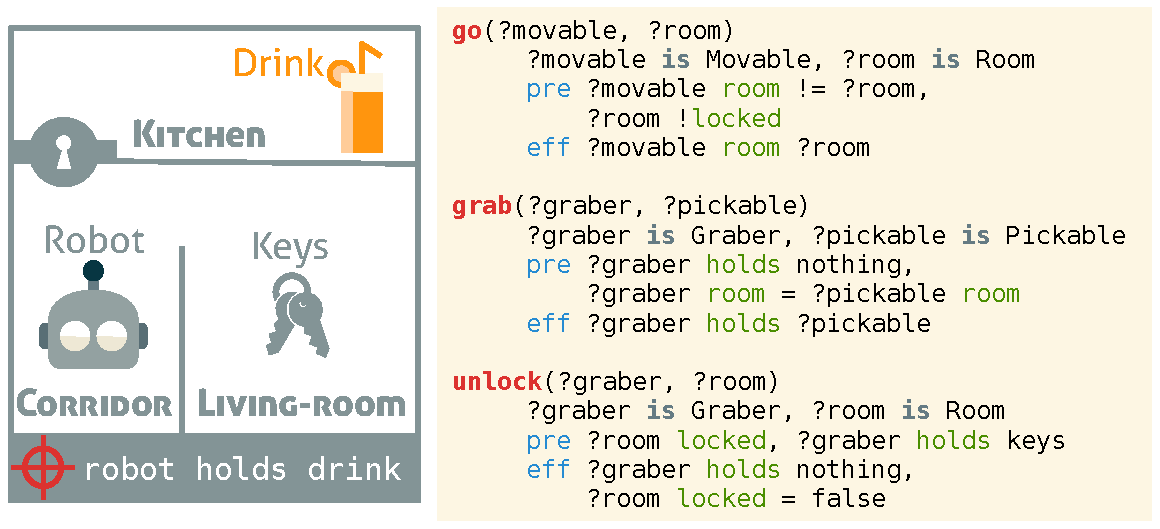
\includegraphics{graphics/example.pdf}
\caption{\label{fig:example}Example domain and problem featuring a robot
that aims to fetch a lollipop in a locked kitchen. The operator
\lstinline!go! is used for movable objects (such as the robot) to move
to another room. The \lstinline!grab! operator is used by grabbers to
hold objects and the \lstinline!unlock! operator is used to open a door
when the robot holds the key.}
\end{figure}

In order to simplify this framework, we need to introduce some
differences from the classical partial plan representation. First, the
partial plan is a part of the problem tuple as it is a needed input of
the LOLLIPOP algorithm.

\begin{definition}[Partial Plan]

We define a partial plan as a tuple \(\langle S, L, B\rangle\) with
\(S\) the set of \textbf{steps} (semi or fully instantiated operators
also called \emph{actions}), \(L\) the set of \textbf{causal links}, and
\(B\) the set of \textbf{binding constraints}.

\end{definition}

Second we factorize the set of \emph{ordering constraints}, used in
classical representations, as being part of the causal links. Indeed,
causal links are always supported by an ordering constraint. The only
case where bare ordering constraints are needed is in threats. We
represent them with \textbf{bare causal links}. These are stored as
causal links without bearing any fluents. Causal links can be
represented by their bore fluents called \emph{causes}. We note
\(f \in l\) the fact that a causal link \(l\) bears the fluent \(f\)
(bare causal links are noted \(l = \emptyset\)). That allows us to
introduce the \textbf{precedence operator} noted \(a_i \succ a_j\) with
\(a_i, a_j \in S\) iff there is a path of causal links that connects
\(a_i\) to \(a_j\). We call \(a_i\) \emph{anterior} to \(a_j\).

A specificity of Partial Order Planning is that it fixes flaws in a
partial plan in order to refine it into a valid plan that is a solution
to the given problem. Next, we define the classical flaws in our
framework.

\begin{definition}[Subgoal]

A flaw in a partial plan, called subgoal, is a missing causal link
required to satisfy a precondition of a step. We can note a subgoal as:
\(a_p \xrightarrow{s} a_n \notin L \mid \{ a_p, a_n \} \subseteq S\)
with \(a_n\) called the \textbf{needer} and \(a_p\) an eventual
\textbf{provider} of the fluent \(s\). This fluent is called \emph{open
condition} or \textbf{proper fluent} of the subgoal.

\end{definition}

\begin{definition}[Threat]

A flaw in a partial plan called threat consists of having an effect of a
step that can be inserted between two actions with a causal link that is
threatened by the said effect. We say that a step \(a_b\) is threatening
a causal link \(a_p \xrightarrow{t} a_n\) iff
\(a_b \neq a_p \neq a_n \land \neg t \in eff(a_b) \land a_p \succ a_b \succ a_n\)
with \(a_b\) being the \textbf{breaker}, \(a_n\) the \emph{needer} and
\(a_p\) a \emph{provider} of the \emph{proper fluent} \(t\).

\end{definition}

Flaws are fixed via the application of a resolver to the plan. A flaw
can have several resolvers that match its needs.

\begin{definition}[Resolvers]\label{def:resolver}

A resolver is a potential causal link defined as a tuple
\(r = \langle a_s, a_t, f\rangle\) with:

\begin{itemize}
\tightlist
\item
  \(a_s, a_t \in S\) being the source and the target of the resolver,
\item
  \(f\) being the considered fluent.
\end{itemize}

\end{definition}

For classical flaws, the resolvers are simple to find. For a
\emph{subgoal} the resolvers are sets of the potential causal links
between a possible provider of the proper fluent and the needer. To
solve a \emph{threat} there are mainly two resolvers: a causal link
between the needer and the breaker called \textbf{demotion} or a causal
link between the breaker and the provider called \textbf{promotion}.

Once the resolver is applied, another important step is needed in order
to be able to keep refining. The algorithm needs to take into account
the \textbf{side effects} the application of the resolver had on the
partial plan. Side effects are searched by type.

\begin{definition}[Side effects]\label{def:sideeffect}

Flaws that arise because of the application of a resolver on the partial
plan are called causal side effects or \emph{related flaws}. They are
caused by an action \(a_t\) called the \textbf{trouble maker} of a
resolver. This action is the \emph{source} of the resolver applied onto
the plan.

\end{definition}

We can derive this definition for subgoals and threats:

\begin{itemize}
\tightlist
\item
  \textbf{Related Subgoals} are all the open conditions inserted with
  the \emph{trouble maker}. The subgoals are often searched using the
  preconditions of the trouble maker and added when no causal links
  satisfy them.
\item
  \textbf{Related Threats} are the causal links threatened by the
  insertion of the \emph{trouble maker}. They are added when there is no
  causal path that prevents the action to interfere with the threatened
  causal link.
\end{itemize}

\begin{figure}[htbp]
\centering
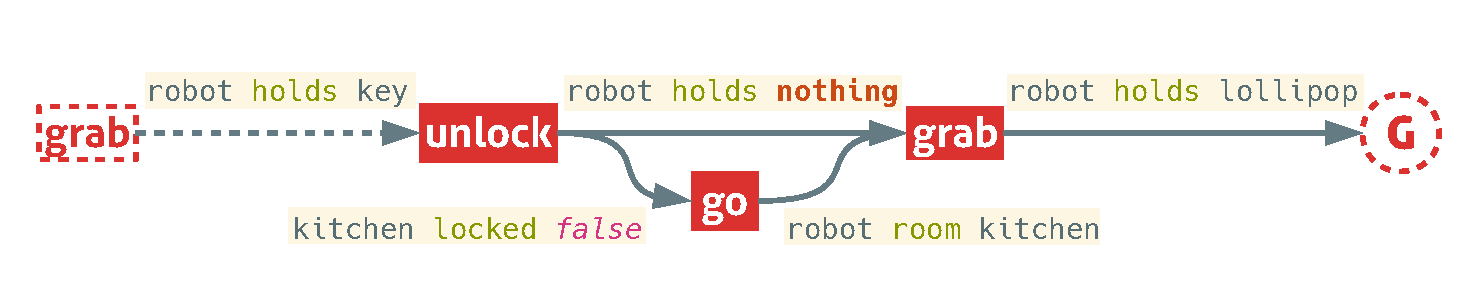
\includegraphics{graphics/partialplan1.pdf}
\caption{\label{fig:partialplan1}Example of a partial plan occurring
during the computation of POP on the previous example domain illustrated
by \cref{fig:example}. Full arrows are existing causal links. The dotted
arrow and operator depict the current resolver.}
\end{figure}

In the partial plan presented in \cref{fig:partialplan1}, we consider
that a resolver providing the fluent \lstinline!robot holds key! is
considered. This resolver will introduce the open conditions
\lstinline!robot holds nothing, key room _room, robot room _room! since
it just introduced this instantiation of the \lstinline!grab! operator
in the partial plan. These will trigger the insertion of a subgoal that
will have this new \lstinline!grab! operator as needer. The potentially
related threat of this resolver is that the effect
\lstinline!robot holds key! might threaten the link between the existing
\lstinline!unlock! and \lstinline!grab! steps, but won't be considered
since there are no way the new step can be inserted after
\lstinline!unlock!.

\subsection{Classical POP Algorithm}\label{classical-pop-algorithm}

The classical POP algorithm is pretty straight forward: it starts with a
simple partial plan and refines its \emph{flaws} until they are all
resolved to make the found plan a solution of the problem.

\begin{algorithm}\caption{Classical Partial Order Planning}\label{alg:pop}\begin{algorithmic}[1]

\footnotesize
\Function{pop}{Queue of Flaws $a$, Problem $\Pi$}
\State \Call{populate}{$a$, $\Pi$}
\Comment{Populate agenda only on first call} \If{$\Pi.G = \emptyset$}
\Comment{Goal is empty, default solution is provided}
\State \(\Pi.p.L \gets (I \rightarrow G)\) \label{line:emptygoal} \EndIf
 \If{$a = \emptyset$} \State \Return Success
\Comment{Stop all recursion} \EndIf
 \State Flaw \(f \gets\) \Call{choose}{$a$} \label{line:flawselection}
\Comment{Non deterministic choice} \State Resolvers \(R \gets\)
\Call{resolvers}{$f$, $\Pi$} \ForAll{$r \in R$}
\Comment{Non deterministic choice operator}
\State \Call{apply}{$r$, $\Pi.p$} \label{line:resolverapplication}
\Comment{Apply resolver to partial plan} \State SideEffects \(s \gets\)
\Call{sideEffect}{$r$} \label{line:sideeffectapplication}
\State \Call{apply}{$s$, $a$} \Comment{Side effects of the resolver}
\If{\protect\Call{pop}{$a$, $\Pi$} = Success}
\Comment{Refining recursively} \State \Return Success \EndIf
 \State \Call{revert}{$r$, $\Pi.p$}
\Comment{Failure, undo resolver insertion}
\State \Call{revert}{$s$, $a$}
\Comment{Failure, undo side effects application} \EndFor
 \State \Return Failure
\Comment{Revert to last non deterministic choice of resolver}
\EndFunction

\end{algorithmic}\end{algorithm}

The algorithm~\ref{alg:pop} is inspired by
{[}\protect\hyperlink{ref-ghallabux5fautomatedux5f2004}{19}{]}. This POP
implementation uses an agenda of flaws that is efficiently updated after
each refinement of the plan. At each iteration, a flaw is selected and
removed from the agenda (line~\ref{line:flawselection}). A resolver for
this flaw is then selected and applied
(line~\ref{line:resolverapplication}). If all resolvers cause failures,
the algorithm backtracks to the last resolver selection to try another
one. The algorithm terminates when no more resolver fits a flaw
(\lstinline!Failure!) or when all flaws have been fixed
(\lstinline!Success!).

This standard implementation has several limitations. First, it can
easily make poor choices that will lead to excessive backtracking. It
also can't undo redundant or non-optimal links if they don't lead to
backtracking. To explain these limitations, we use the example described
in \cref{fig:example} where a robot must fetch a lollipop in a locked
room. This problem is solvable by regular POP algorithms. However, we
can have some cases where small changes in POP's inputs can cause a lot
of unnecessary back-tracking. For example, if we add a new action called
\lstinline!dig_through_wall! that has as effect to be in the desired
room but that requires a \emph{jackhammer}, the algorithm will simply
need more backtracking. The effects could be worse if obtaining a
jackhammer would require numerous steps (for example needing to build
it). This problem can be solved most of the time using simple flaw
selection mechanisms. The other limitation arises when the plan has been
modified. This can arise in the context of dynamic environments of
online planning applications. When POP is modified to use input plans
{[}\protect\hyperlink{ref-sebastiaux5fgraph-basedux5f2000}{20}{]}, these
partial plans are carefully designed not to infringe the properties
required by POP to operate. In our case, the plan can contain misleading
information and this can cause a variety of new problems that can only
be fixed using new refinements methods.

\section{LOLLIPOP's Approach}\label{lollipops-approach}

LOLLIPOP makes use of proper plans in order to ease the initial
backchaining of POP and to drive the flaw and resolver selection,
including the new negative flaws we introduced for online planning
refinements.

\subsection{Proper Plan Generation}\label{sec:properplan}

One of the main contributions of the present paper is our use of the
concept of \emph{proper plan}. First of all, we define this notion.

\begin{definition}[Proper Plan]

A proper plan \(O^P\) of a set of operators \(O\) is a labeled directed
graph that binds two operators with the causal link
\(o_1 \xrightarrow{f} o_2\) iff it exists at least a unifying fluent
\(f \in eff(o_1) \cap pre(o_2)\).

\end{definition}

This definition was inspired by the notion of domain causal graph as
explained in
{[}\protect\hyperlink{ref-gobelbeckerux5fcomingux5f2010}{18}{]} and
originally used as heuristic in
{[}\protect\hyperlink{ref-helmertux5ffastux5f2006}{21}{]}. Causal graphs
have fluents as their nodes and operators as their edges. Proper plans
are the opposite: an \emph{operator dependency graph} for a set of
actions. A similar structure was used in
{[}\protect\hyperlink{ref-smithux5fpostponingux5f1993}{22}{]} that
builds the operator dependency graph of goals and uses precondition
nodes instead of labels. This structure is very useful for getting
information on the \emph{shape of a problem}. This shape leads to an
intuition based on the potential usefulness or hurtfulness of operators.
Cycles in this graph denote the dependencies of operators. We call
\emph{co-dependent} operators that form a cycle. If the cycle is made of
only one operator (self-loop), then it is called \emph{auto-dependent}.

While building this proper plan, we need a \textbf{providing map} that
indicates, for each fluent, the list of operators that can provide it.
This is a simpler version of the causal graphs that is reduced to an
associative table easier to update. The list of providers can be sorted
in order to drive resolver selection (like detailed in
\cref{sec:selection}). A \textbf{needing map} is also built but is only
used for proper plan generation. We note \(\Delta^P\) the proper plan
built with the set of operators in the domain \(\Delta\). In the
\cref{fig:properplan}, we illustrate the application of this mechanism
on our example from \cref{fig:example}. Continuous lines correspond the
\emph{domain proper plan}.

\begin{figure}[htbp]
\centering
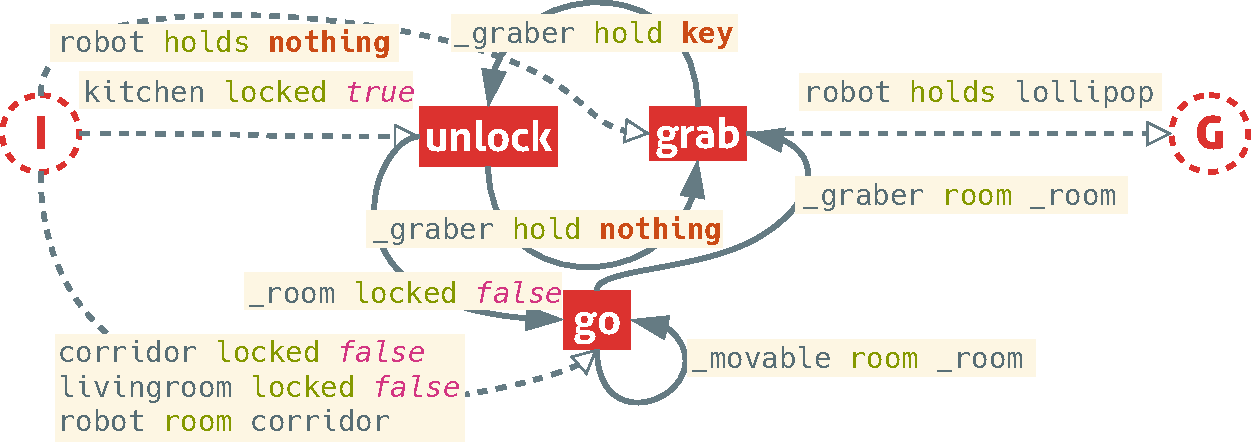
\includegraphics{graphics/properplan.pdf}
\caption{\label{fig:properplan}Diagram of the proper plan of example
domain. In full arrows the proper plan computed during domain
compilation time and in dotted arrows the dependencies are added to
inject the initial and goal steps.}
\end{figure}

The generation of the proper plan is based upon the previous definition.
It will explore the operators space and build a providing and needing
map that gives the provided and needed fluents for each operator. Once
done it iterates on every precondition and search for a satisfying cause
in order to add the causal links to the proper plan. The
algorithm~\ref{alg:properplan} details this procedure.

\begin{algorithm}\caption{Proper plan generation and update algorithm}\label{alg:properplan}\begin{algorithmic}[1]

\footnotesize
\Function{addVertex}{Operator $o$} \State \Call{cache}{$o$}
\Comment{Update of the providing and needing map} \If {binding}
\Comment{boolean that indicates if the binding was requested}
\State \Call{bind}{$o$} \EndIf
\EndFunction
\Function{cache}{Operator $o$} \ForAll{$eff \in eff(o)$}
\Comment{Adds $o$ to the list of providers of $eff$}
\State \Call{add}{$providing, eff, o$} \EndFor
 \State \ldots{} \Comment{Same operation with needing and preconditions}
\EndFunction
\Function{bind}{Operator $o$} \ForAll{$pre \in pre(o)$}
\If{$pre \in providing$} \ForAll{$p \in$ \Call{get}{$providing$, $pre$}}
\State Link \(l \gets\) \Call{getEdge}{$p$, $o$}
\Comment{Create the link if needed} \State \(l \gets l \cup \{pre\}\)
\Comment{Add the fluent as a cause} \EndFor
 \EndIf
 \EndFor
 \State \ldots{} \Comment{Same operation with needing and effects}
\EndFunction

\end{algorithmic}\end{algorithm}

Applying the notion of proper plan for problems only needs the initial
and goal steps added in the proper plan. In \cref{fig:properplan}, we
depict this insertion with our previous example using dotted lines.
However, since proper plans feature cycles, they can't be used directly
as input to POP algorithms to ease the initial backchaining. Moreover,
the process of refining a proper plan into a usable one could be more
computationally expensive than POP itself.

In order to give a head start to the LOLLIPOP algorithm, we propose to
build proper plans differently with the algorithm detailed in
algorithm~\ref{alg:safeproperplan}. A similar notion was already
presented as ``basic plans'' in
{[}\protect\hyperlink{ref-sebastiaux5fgraph-basedux5f2000}{20}{]}. These
partial plans uses a more complete but slower solution for generation
that ensures that each selected steps is \emph{necessary} for the
solution. In our case, we built a simpler solution that can solve some
basic planning problems but that also make early assumption (since our
algorithm can handle them). It does a simple and fast backward
construction of a partial plan driven by the providing map. Therefore,
it can be tweaked with the powerful heuristics of state search planning.

\begin{algorithm}\caption{Safe proper plan generation algorithm}\label{alg:safeproperplan}\begin{algorithmic}[1]

\footnotesize
\Function{safe}{Problem $\Pi$} \State Stack \(open \gets [\Pi.G]\)
\State Stack \(closed \gets \emptyset\) \While{$open \neq \emptyset$}
\State Operator \(o \gets\) \Call{pop}{$open$}
\Comment{Remove $o$ from $open$} \State \Call{push}{$closed$, $o$}
\ForAll {$pre \in pre(o)$} \State Operators \(p \gets\)
\Call{getProviding}{$\pi$, $pre$} \Comment{Sorted by usefulness}
\If{$p = \emptyset$} \Comment{(see section~\ref{sec:selection})}
\State \(\Pi.p.S \gets \Pi.p.S \setminus \{p\}\) \Continue
 \EndIf
 \State Operator \(o' \gets\) \Call{getFirst}{$p$}
\label{line:safefirst} \If{$o' \in closed$} \Continue
 \EndIf
 \If{$o' \not \in \Pi.p.S$} \State \Call{push}{$open$, $o'$} \EndIf
 \State \(\Pi.p.S \gets \Pi.p.S \cup \{o'\}\) \State Link \(l \gets\)
\Call{getEdge}{$o'$, $o$} \Comment{Create the link if needed}
\State \(l \gets l \cup \{pre\}\) \Comment{Add the fluent as a cause}
\EndFor
 \EndWhile
\EndFunction

\end{algorithmic}\end{algorithm}

This algorithm is very useful since it is specifically used on goals.
The result is a valid partial plan that can be used as input to POP
algorithms.

\subsection{Negative Refinements and Plan
Optimization}\label{sec:negative}

Classical POP algorithm works upon a principle of positive plan
refinements. The two standard flaws (subgoals and threats) are fixed by
\emph{adding} steps, causal links, or variable binding constraints to
the partial plan. Online planning needs to be able to \emph{remove} part
of the plan that isn't necessary for the solution. Since we assume that
the input partial plan is quite complete, we need to define new flaws to
optimize and fix this plan. These flaws are called \emph{negative} as
their resolvers apply subtractive refinements on partial plans.

\begin{definition}[Alternative]\label{def:alternative}

An alternative is a negative flaw that occurs when it exists a better
provider choice for a given link. An alternative to a causal link
\(a_p \xrightarrow{f} a_n\) is a provider \(a_b\) that has a better
\emph{utility value} than \(a_p\).

\end{definition}

The \textbf{utility value} of an operator is a measure of usefulness at
the heart of our ranking mechanism detailed in \cref{sec:selection}. It
uses the incoming and outgoing degrees of the operator in the domain
proper plan to measure its usefulness.

Finding an alternative to an operator is computationally expensive. It
requires searching a better provider for every fluent needed by a step.
In order to simplify that search, we select only the best provider for a
given fluent and check if the one used is the same one. If not, we add
the alternative as a flaw. This search is done only on updated steps for
online planning. Indeed, the safe proper plan mechanism is guaranteed to
only choose the best provider (algorithm~\ref{alg:safeproperplan} at
line~\ref{line:safefirst}). Furthermore, subgoals won't introduce new
fixable alternative as they are guaranteed to select the best possible
provider.

\begin{definition}[Orphan]

An orphan is a negative flaw that means that a step in the partial plan
(other than the initial or goal step) is not participating in the plan.
Formally, \(a_o\) is an orphan iff
\(a_o \neq I \land a_o \neq G \land \left( p.d^+(a_o) = 0 \right) \lor \forall l \in p.L^+(a_o), l=\emptyset\).

\end{definition}

With \(p.d^+(a_o)\) being the \emph{outgoing degree} of \(a_o\) in the
directed graph formed by \(p\) and \(p.L^+(a_o)\) being the set of
\emph{outgoing causal links} of \(a_o\) in \(p\). This last condition
checks for \emph{hanging orphans} that are bound with the goal with only
bare causal links introduced by threat resolution.

The introduction of negative flaws requires modifying the resolver
definition (cf. definition~\ref{def:resolver}).

\begin{definition}[Signed Resolvers]

A signed resolver is a resolver with a notion of sign. We add to the
resolver tuple the sign of the resolver noted \(s \in \{+, -\}\).

\end{definition}

The previously defined negative flaws have all their associated negative
resolvers. The solution to an alternative is a negative refinement that
simply removes the targeted causal link. This causes a new subgoal as a
side effect, that will prioritize its resolver by its rank (explained in
\cref{sec:selection}) and then pick the first provider (the most useful
one). The resolver for orphans is the negative refinement that is meant
to remove a step and its incoming causal link while tagging its
providers as potential orphans.

\begin{figure}[htbp]
\centering
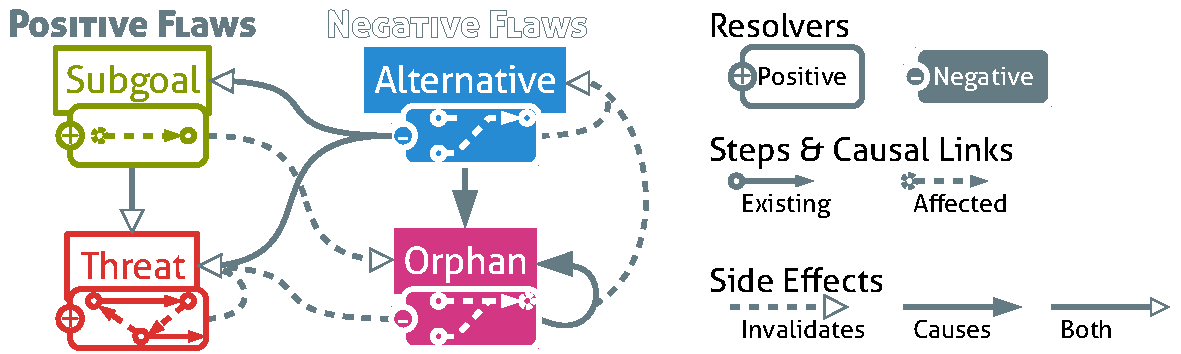
\includegraphics{graphics/sideeffects.pdf}
\caption{\label{fig:sideeffects}Schema representing flaws with their
signs, resolvers and side effects relative to each other}
\end{figure}

The side effect mechanism also needs an upgrade since the new kind of
flaws can easily interfere with one another. This is why we extend the
side effect definition (definition~\ref{def:sideeffect}) with a notion
of sign.

\begin{definition}[Signed Side Effects]

A signed side effect is either a regular \emph{causal side effect} or an
\emph{invalidating side effect}. The sign of a side effect indicates if
the related flaw needs to be added or removed from the agenda.

\end{definition}

The \cref{fig:sideeffects} exposes the extended notion of signed
resolvers and side effects. When treating positive resolvers, nothing
needs to change from the classical method. When dealing with negative
resolvers, we need to search for additional subgoals and threats.
Deletion of causal links and steps can cause orphan flaws that need to
be identified for removal.

In {[}\protect\hyperlink{ref-peotux5fthreatremovalux5f1993}{23}{]}, a
\textbf{invalidating side effect} is explained under the name of
\emph{DEnd} strategy. In classical POP, it has been noticed that threats
can disappear in some cases if subgoals or other threats were applied
before them. For our formalism, we decide to gather under this notion
every side effects that removes the need to consider a flaw. For
example, orphans can be ``saved'' if a subgoal selects the orphan step.
Alternatives can remove the need to compute further subgoal of a now
orphan step as orphans simply remove the need to fix any flaws that
concern the selected step.

These interactions between flaws are decisive in the validity and
efficiency of the whole model, that is why we aim to drive flaw
selection in a very rigorous manner.

\subsection{Driving Flaws and Resolvers Selection}\label{sec:selection}

Resolvers and flaws selection are the keys to improving performances.
Choosing a good resolver helps to reduce the branching factor that
accounts for most of the time spent on running POP algorithms
{[}\protect\hyperlink{ref-kambhampatiux5fdesignux5f1994}{24}{]}. Flaw
selection is also very important for efficiency, especially when
considering negative flaws which can conflict with other flaws.

Conflicts between flaws occur when two flaws of opposite sign target the
same element of the partial plan. This can happen for example if an
orphan removes a step needed by a subgoal or when a threat tries to add
a promoting link against an alternative. The use of side effects will
prevent most of these occurrences in the agenda but a base ordering will
increase the general efficiency of the algorithm.

Based on the \cref{fig:sideeffects}, we create a base ordering of flaws
by type. This order takes into account the number of flaw types affected
by causal side effects.

\begin{enumerate}
\def\labelenumi{\arabic{enumi}.}
\tightlist
\item
  \textbf{Alternatives} will cut causal links that have a better
  provider. It is necessary to identify them early since they will add
  at least another subgoal to be fixed as a related flaw.
\item
  \textbf{Subgoals} are the flaws that cause most of the branching
  factor in POP algorithms. This is why we need to make sure that all
  open conditions are fixed before proceeding on finer refinements.
\item
  \textbf{Orphans} remove unneeded branches of the plan. However, these
  branches can be found out to be necessary for the plan in order to
  meet a subgoal. Since a branch can contain numerous actions, it is
  preferable to let the orphan in the plan until they are no longer
  needed. Also, threats concerning orphans are invalidated if the orphan
  is resolved first.
\item
  \textbf{Threats} occur quite often in the computation. They cost a lot
  of processing power since they need to check if there are no paths
  that fix the flaw already. Numerous threats are generated without the
  need of intervention
  {[}\protect\hyperlink{ref-peotux5fthreatremovalux5f1993}{23}{]}. That
  is why we prioritize all related subgoals and orphans before threats
  because they can add causal links or remove threatening actions that
  will fix the threat.
\end{enumerate}

Resolvers need to be ordered as well, especially for the subgoal flaw.
Ordering resolvers for a subgoal is the same operation as choosing a
provider. Therefore, the problem becomes ``how to rank operators?''. The
most relevant information on an operator is its usefulness and
hurtfulness. These indicate how much an operator will help and how much
it may cause branching after selection.

\begin{definition}[Degree of an operator]

Degrees are a measurement of the usefulness of an operator. The notion
is derived from the incoming and outgoing degrees of a node in a graph.

We note \(p.d^+(o)\) and \(p.d^-(o)\) respectively the outgoing and
incoming degrees of an operator in a plan \(p\). These represent the
number of causal links that goes out or toward the operator. We call
proper degree of an operator \(o.d^+ = |eff(o)|\) and
\(o.d^- = |pre(o)|\) the number of preconditions and effects that
reflects its intrinsic usefulness.

\end{definition}

There are several ways to use the degrees as indicators. \emph{Utility
value} increases with every \(d^+\), since this reflects a positive
participation in the plan. It decreases with every \(d^-\) since actions
with higher incoming degrees are harder to satisfy. The utility value
bounds are useful when selecting special operators. For example, a
user-specified constraint could be laid upon an operator to ensure it is
only selected as a last resort. This operator will be affected with the
minimum value for the utility value. More commonly, the maximum value is
used for initial and goal step to ensure their selection.

Our ranking mechanism includes several computation steps. The first step
is the computation of the \textbf{base scores} noted
\(Z_0(o)=\langle o^+, o^-\rangle\). It is a tuple that contains two
components: a positive score that acts as a participation measurement
and a negative score that represents the dependencies of the operator.
For each component of the score we consider a \emph{sub score array}
noted \(S_z(o^\pm)\). We define them as follows:

\begin{itemize}
\tightlist
\item
  \(S_z(o^+)\) containing only \(\Delta^P.d^+(o)\), the positive degree
  of \(o\) in the domain proper plan. This will give a measurement of
  the predicted usefulness of the operator.
\item
  \(S_z(o^-)\) containing the following sub-scores:

  \begin{enumerate}
  \def\labelenumi{\arabic{enumi}.}
  \tightlist
  \item
    \(o.d^-\) the proper negative degree of \(o\). Having more
    preconditions can lead to a potentially higher need for subgoals.
  \item
    \(\sum_{c \in C_{\Delta^P}(o)}|c|\) with \(C_{\Delta^P}(o)\) being
    the set of cycles where \(o\) participates in the domain proper
    plan. If an action is co-dependent it may lead to a dead end when
    searching for precondition as it will form a cycle.
  \item
    \(|SC(o)|\) with \(SC(o)\) is the set of self-cycle \(o\)
    participates in. This is usually symptomatic of a \emph{toxic
    operator} (cf. definition~\ref{def:toxic}). Having an operator
    behaving this way can lead to problems in the operator
    instantiation.
  \item
    \(\left|pre(o) \setminus \Delta^P.L^-(o)\right|\) with
    \(\Delta^P.L^-(o)\) being the set of incoming edges of \(o\) in the
    proper plan of the domain. This represents the number of open
    conditions in the domain proper plan. This is symptomatic of action
    that can't be satisfied without a compliant initial step.
  \end{enumerate}
\end{itemize}

A parameter is reserved for each sub-score. It is noted \(P_n^\pm\) with
\(n\) being the index of the subgoal in the list. The final formula for
the score is then defined as:
\(o^\pm = \sum_{n=1}^{|S_z(o^\pm)|}{P_n^\pm S_z^n(o^\pm)}\)

Once this score is computed, the ranking mechanism starts the second
phase, it computes the \textbf{realization scores} that are potential
scores that are realized once the problem is specified. It first
searches the \emph{inapplicable operators} that are all operators in the
domain proper plan that have a precondition that isn't satisfied with a
causal link. Then it searches the \emph{eager operators} that provide
fluents with no corresponding causal link (as they are not needed).
These operators are stored in relation with their inapplicable or eager
fluents.

The third phase starts with the beginning of the solving algorithm, once
the problem has been provided. It computes the \emph{effective
realization scores} based on the initial and goal step. It will add
\(P_1^+\) to \(o^+\) for each realized eager operators (if the goal
contains the related fluent) and subtract \(P_4^-\) from \(o^-\) for
each inapplicable operators realized by the initial step.

Last, the \textbf{final score} of each operator \(o\), noted \(r_o\), is
computed from positive and negative scores using the following formula:
\(r_o = o^+ \alpha^{-o^-}\). This respects the criteria of having a
bounded value for the \emph{utility value} as it ensures that the value
is positive with \(0\) as a minimum bound and \(+\infty\) for a maximum.
The initial and goal steps have their utility value set to the upper
bound in order to ensure their selection of other steps.

Choosing to compute the resolver selection at operator level has some
interesting consequences on the performances. Indeed, this computation
is much lighter than approaches with heuristics on plan space
{[}\protect\hyperlink{ref-shekharux5flearningux5f2016}{14}{]} as it
reduce the overhead caused by real time computation of heuristics on
complex data. In order to reduce this overhead more, the algorithm sorts
the providing associative array in order to easily retrieve the best
operator for each fluent. This means that the evaluation of the
heuristic is done only once for each operator. This reduces the overhead
and allows for faster results on smaller plans.

\subsection{LOLLIPOP Algorithm}\label{sec:algorithm}

The LOLLIPOP algorithm uses the same refinement algorithm as described
in algorithm~\ref{alg:pop}. The differences reside in the changes made
on the notions of resolvers and side effects. In
line~\ref{line:resolverapplication} of algorithm~\ref{alg:pop}, LOLLIPOP
algorithm will apply negative resolvers if the selected flaw is
negative. In line~\ref{line:sideeffectapplication}, it will search for
both sign of side effects. Another change resides in the initialization
of the solving mechanism and the domain as detailed in
algorithm~\ref{alg:lollipopinit}. This algorithm contains several parts.
First, the \textproc{domainInit} function corresponds to the code
computed during the domain compilation time. It will prepare the
rankings, the proper plan and its caching mechanisms. It will also use
strongly connected component detection algorithm to detect cycles. These
cycles are used during the base score computation
(line~\ref{line:basescore}). We added a detection of illegal fluents and
operators in our domain initialization (line~\ref{line:isillegal}).
Illegal operators are either inconsistent or toxic.

\begin{algorithm}\caption{LOLLIPOP initialization mechanisms}\label{alg:lollipopinit}\begin{algorithmic}[1]

\footnotesize
\Function{domainInit}{Operators $O$} \State ProperPlan \(P\)
\State Ranking \(R\) \ForAll{Operator $o \in O$}
\If{\Call{isIllegal}{$o$}} \Comment{Remove toxic and useless fluents}
\label{line:isillegal} \State \(O \gets O \setminus \{o\}\)
\Comment{If entirely toxic or useless} \Continue
 \EndIf
 \State \(P.\)\Call{addVertex}{$o$}
\Comment{Add, cache and bind all operators} \EndFor
 \State Cycles \(C \gets\) \Call{stronglyConnectedComponent}{$P$}
\Comment{Using DFS} \State \(R.Z \gets\) \Call{baseScores}{$O$, $P$}
\label{line:basescore} \State \(R.I \gets\) \Call{inapplicables}{$P$}
\State \(R.E \gets\) \Call{eagers}{$P$} \EndFunction
\Function{lollipopInit}{Problem $\Pi$}
\State \Call{realize}{$\Pi.\Delta.R, \Pi$} \Comment{Realize the scores}
\State \Call{cache}{$\Pi.\Delta.P, \Pi.I$}
\Comment{Cache initial step in providing …}
\State \Call{cache}{$\Pi.\Delta.P, \Pi.G$}
\Comment{… as well as goal step}
\State \Call{sort}{$\Pi.\Delta.P.providing$, $\Pi.\Delta.R$}
\Comment{Sort the providing map} \If{$\Pi.p.L = \emptyset$}
\State \Call{safe}{$\Pi$}
\Comment{Computing the safe proper plan if the plan is empty} \EndIf
 \State \Call{populate}{$a$, $\Pi$}
\Comment{populate agenda with first flaws} \label{line:populate}
\EndFunction
\Function{populate}{Agenda $a$, Problem $\Pi$}
\ForAll{Update $u \in \Pi.U$} \Comment{Updates due to online planning}
\State Fluents \(F \gets eff(u.new) \setminus eff(u.old)\)
\Comment{Added effects} \ForAll{Fluent $f \in F$}
\ForAll{Operator $o \in$ \Call{better}{$\Pi.\Delta.P.providing$, $f$, $o$}}
\ForAll{Link $l \in \Pi.P.L^+(o)$} \If{$f \in l$}
\State \Call{addAlternative}{$a$, $f$, $o$, $\rightarrow(l)$, $\Pi$}
\State \Comment{With $\rightarrow(l)$ the target of $l$} \EndIf
 \EndFor
 \EndFor
 \EndFor
 \State \(F \gets eff(u.old) \setminus eff(u.new)\)
\Comment{Removed effects} \ForAll{Fluent $f \in F$}
\ForAll{Link $l \in \Pi.P.L^+(u.new)$} \If{\Call{isLiar}{$l$}}
\State \(\Pi.L \gets \Pi.L \setminus \{l\}\)
\State \Call{addOrphans}{$a$, $u.new$, $\Pi$} \EndIf
 \EndFor
 \EndFor
 \State \ldots{}
\Comment{Same with removed preconditions and incomming liar links}
\EndFor
 \ForAll{Operator $o \in \Pi.p.S$}
\State \Call{addSubgoals}{$a$, $o$, $\Pi$}
\State \Call{addThreats}{$a$, $o$, $\Pi$} \EndFor
\EndFunction

\end{algorithmic}\end{algorithm}

\begin{definition}[Inconsistent operators]

An operator \(a\) is contradictory iff
\(\exists f \{f, \lnot f \} \in eff(o) \lor \{f, \lnot f \} \in pre(o)\)

\end{definition}

\begin{definition}[Toxic operators]\label{def:toxic}

Toxic operators have effects that are already in their preconditions or
empty effects. An operator \(o\) is toxic iff
\(pre(o) \cap eff(o) \neq \emptyset \lor eff(o) = \emptyset\)

\end{definition}

Toxic actions can damage a plan as well as make the execution of POP
algorithm longer than necessary. This is fixed by removing the toxic
fluents (\(pre(a) \nsubseteq eff(a)\)) and by updating the effects with
\(eff(a) = eff(a) \setminus pre(a)\). If the effects become empty, the
operator is removed from the domain.

The \textproc{lollipopInit} function is executed during the
initialization of the solving algorithm. We start by realizing the
scores, then we add the initial and goal step in the providing map by
caching them. Once the ranking mechanism is ready, we sort the providing
map. With the ordered providing map the algorithm runs the fast
generation of the safe proper plan for the problem's goal.

The last part of this initialization (line~\ref{line:populate}) is the
agenda population that is detailed in the \textproc{populate} function.
During this step, we perform a search of alternatives based on the list
of updated fluents. A big problem with online updates is that the plan
can become outdated relative to the domain.

\begin{definition}[Liar links]

A liar link is a link that doesn't hold a fluent in the preconditions or
effect of its source and target. We note:
\[a_i \xrightarrow{f} a_j | f \notin eff(a_i) \cap pre(a_j)\]

\end{definition}

A liar link can be created by the removal of an effect or preconditions
during online updates (with the causal link still remaining).

We call lies, fluents that are held by links without being in the
connected operators. To resolve the problem we remove all lies. We
delete the link altogether if it doesn't bear any fluent as a result of
this operation. This removal triggers the addition of orphan flaws.

While updated operators is very important for LOLLIPOP to be able to
solve online planning problems, another mechanism is used in order to
ensure that LOLLIPOP is complete. This mechanism is explained in
lemma~\ref{lem:deadend-validity}.

\section{Theoretical Analysis}\label{sec:analysis}

As proven in
{[}\protect\hyperlink{ref-penberthyux5fucpopux5f1992}{8}{]}, the
classical POP algorithm is \emph{sound} and \emph{complete}. In order to
prove that these properties apply to LOLLIPOP, we need to introduce some
hypothesis:

\begin{itemize}
\tightlist
\item
  operators updated by online planning are known.
\item
  user provided steps are known.
\item
  user provided plans don't contain illegal artifacts. This includes
  toxic or inconsistent actions, lying links and cycles.
\end{itemize}

First, we define some additional properties of partial plans.

\begin{definition}[Full Support]\label{def:fullsupport}

A partial plan \(p\) is fully supported if each of its steps
\(o \in p.S\) is fully supported. A step is fully supported if each of
its preconditions \(f \in pre(o)\) is supported. A precondition is fully
supported if it exists a causal link \(l\) that provides it. We note:
\[fs(p) \equiv
\begin{array}{l}
    \forall o \in p.S \thickspace \forall f \in pre(o) \thickspace \exists l \in p.L^-(o): \\
        \left(f \in l \land \not \exists t \in p.S (l_{\rightarrow} \succ t \succ o \land \lnot f \in eff(t))\right)
\end{array}\] with \(p.L^-(o)\) being the incoming causal links of \(o\)
in \(p\) and \(l_{\rightarrow}\) being the source of the link.

\end{definition}

The following property is taken from the original proof. We present it
again for convenience.

\begin{definition}[Partial Plan Validity]\label{def:partialplanvalidity}

A partial plan is a \textbf{valid solution} of a problem \(\Pi\) iff it
is \emph{fully supported} and \emph{contains no cycles}. The validity of
\(p\) regarding a problem \(\Pi\) is noted
\(p \models \Pi \equiv fs(p) \land \left(C(p) = \emptyset \right)\) with
\(C(p)\) being the set of cycles in \(p\).

\end{definition}

\subsection{Proof of Soundness}\label{proof-of-soundness}

Based on the definition~\ref{def:partialplanvalidity} we state that:
\begin{equation}
\left(
\begin{array}{l}
    \forall pre \in pre(\Pi.G): \\
    fs(pre) \land
    \begin{array}{l}
        \forall o \in \Pi.L^-_{\rightarrow}(\Pi.G) \thickspace \forall pre' \in pre(o): \\
        \left(fs(pre')\land C_p(o) = \emptyset\right)
    \end{array}
\end{array}
\right) \implies p \models \Pi\label{eq:recursivevalidity}\end{equation}
where \(\Pi.L^-_{\rightarrow}(\Pi.G)\) is the set of direct antecedents
of \(\Pi.G\) and \(C_p(o)\) is the set of fluents containing \(o\) in
\(p\).

This means that \(p\) is a solution if all preconditions of \(G\) are
satisfied. We can satisfy these preconditions using operators iff their
precondition are all satisfied and if there is no other operator that
threatens their supporting links.

First, we need to prove that \cref{eq:recursivevalidity} holds on
LOLLIPOP initialization. We use our hypothesis to rule out the case when
the input plan is invalid. The algorithm~\ref{alg:safeproperplan} will
only solve open conditions in the same way subgoals do it. Therefore,
safe proper plans are valid input plans.

Since the soundness is proven for regular refinements and flaw
selection, we need to consider the effects of the added mechanisms of
LOLLIPOP. The newly introduced refinements are negative, they don't add
new links:

\begin{equation}\forall f \in F(p) \thickspace \forall r \in r(f): C_p(f.n) = C_{f(p)}(f.n)\label{eq:nocycle}\end{equation}
with \(F(p)\) being the set of flaws in \(p\), \(r(f)\) being the set of
resolvers of \(f\), \(f.n\) being the needer of the flaw and \(f(p)\)
being the result partial plan after application of the flaw. Said
otherwise, an iteration of LOLLIPOP won't add cycles inside a partial
plan.

The orphan flaw targets steps that have no path to the goal and
therefore can't add new open conditions or threats. The alternative
targets existing causal links. Removing a causal link in a plan breaks
the full support of the target step. This is why an alternative will
always insert a subgoal in the agenda corresponding to the target of the
removed causal link. Invalidating side effects also don't affect the
soundness of the algorithm since the removed flaws are already solved.
This makes: \begin{equation}
\forall f \in F^-(p): fs(p) \implies fs(f(p))
\label{eq:conssupport}\end{equation} with \(F^-(p)\) being the set of
negative flaws in the plan \(p\). This means that negative flaws don't
compromise the full support of the plan.

\Cref{eq:nocycle,eq:conssupport} leads to \cref{eq:recursivevalidity}
being valid after the execution of LOLLIPOP. The algorithm is,
therefore, sound.

\subsection{Proof of Completeness}\label{proof-of-completeness}

The soundness proof shows that LOLLIPOP's refinements don't affect the
support of plans in term of validity. It was proven that POP is
complete. There are several cases to explore in order to transpose the
property to LOLLIPOP:

\begin{lemma}[Conservation of Validity]

If the input plan is a valid solution, LOLLIPOP returns a valid
solution.

\end{lemma}

\begin{proof}

With \cref{eq:nocycle,eq:conssupport} and the previous proof, the
conservation of validity is already proved. \qedhere

\end{proof}

\begin{lemma}[Reaching Validity with incomplete partial plans]\label{lem:incompletevalidity}

If the input plan is incomplete, LOLLIPOP returns a valid solution.

\end{lemma}

\begin{proof}

Since POP is complete and the \cref{eq:conssupport} proves the
conservation of support by LOLLIPOP, then the algorithm will return a
valid solution if the provided plan is an incomplete plan and the
problem solvable. \qedhere

\end{proof}

\begin{lemma}[Reaching Validity with empty partial plans]

If the input plan is empty, LOLLIPOP returns a valid solution.

\end{lemma}

\begin{proof}

This is proven using lemma~\ref{lem:incompletevalidity} and POP's
completeness. However, we want to add a trivial case to the proof:
\(pre(G) = \emptyset\). In this case the line~\ref{line:emptygoal} of
the algorithm~\ref{alg:pop} will return a valid plan. \qedhere

\end{proof}

\begin{lemma}[Reaching Validity with a dead-end partial plan]\label{lem:deadend-validity}

If the input plan is in a dead-end, LOLLIPOP returns a valid solution.

\end{lemma}

\begin{proof}

Using input plans that can be in a undermined state is not covered by
the original proof. The problem lies in the existing steps in the input
plan. However, using our hypothesis we can add a failure mechanism that
makes LOLLIPOP complete. On failure, the needer of the last flaw is
deleted if it wasn't added by LOLLIPOP. User defined steps are deleted
until the input plan acts like an empty plan. Each deletion will cause
corresponding subgoals to be added to the agenda. In this case, the
backtracking is preserved and all possibilities are explored as in POP.
\qedhere

\end{proof}

As all cases are covered, these proofs show that LOLLIPOP is complete.

\section{Experimental Results}\label{sec:results}

The experimental results were focused around the properties of the
algorithm for online planning. Since classical POP is unable to perform
online planning, we tested our algorithm in relation to the time taken
for solving the problem for the first time. We profiled the algorithm on
a benchmark problem containing each of the possible issues described
previously.

\begin{table}\footnotesize
\centering

\caption{\label{tbl:results}Average times of \(1.000\) executions on the
problem. First column is for a simple run on the problem. Second and
third columns are experiments with one and two changes in the plan after
a first solving. }

\begin{tabular}{@{}llll@{}}
\toprule

\textbf{Experiment} & \emph{Single} & \emph{Online 1} & \emph{Online
2} \\\midrule

\textbf{Time (\(ms\))} & \(0.86937\) & \(0.38754\) & \(0.48123\) \\

\bottomrule
\end{tabular}

\end{table}

The measurements exposed in table X was made with an Intel® Core™
i7-4720HQ with a 2.60GHz clock. Only one core was used for the solving.
The same experiment done only with the measurement code gave a result of
\(70 ns\) of error. We can see an increase of performance in the online
runs because of the way they are conducted by LOLLIPOP.

\begin{figure}[htbp]
\centering
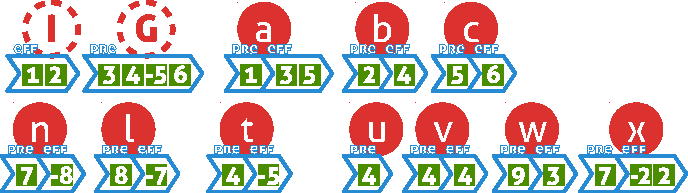
\includegraphics{graphics/experiment.pdf}
\caption{\label{fig:experiment}Domain used to compute the results. First
line is the initial and goal step along with the useful actions. Second
line contains a threatening action \(t\), two co-dependent actions \(n\)
and \(l\), a useless action \(u\), a toxic action \(v\), a deadend
action \(w\) and an inconsistent action \(x\)}
\end{figure}

In \cref{fig:experiment}, we expose the planning domain used for the
experiments. During the domain initialization the action \(u\) and \(v\)
are eleminated from the domain since they serve no purpose in the
solving process. The action \(x\) is stripped of its negative effect
\(-2\) because it is inconsistent with the effect \(2\).

\begin{minipage}{\linewidth}

\begin{lstlisting}
[DEBUG] A(⊧[4]) is useless ! Getting rid of it.
[DEBUG] A(⊧[4]+[4]) is entirely toxic ! Getting rid of it.
\end{lstlisting}

\end{minipage}

\section*{Conclusion}\label{conclusion}
\addcontentsline{toc}{section}{Conclusion}

We proved that LOLLIPOP is sound and complete like POP. It also can be
used for online planning and can refine plans further than POP with
negative refinements that allow it to optimize plans that are already
solution to the problem. These properties make LOLLIPOP suitable for use
in dynamic environments often encountered in robotic applications.

For future works we aim to improve the performance of our algorithm and
its expressiveness in order to represent complex real life problems
encountered by dependent persons. We also aim to develop a soft solving
mechanism that aims to give the best probable plan in case of having an
unsolvable problem. Once ready this planner will be used for plan
recognition using inverted planning.

\textbf{\#TODO Say that we are too shameful to release the source code
to the public}

\section*{References}\label{references}
\addcontentsline{toc}{section}{References}

\hypertarget{refs}{}
\hypertarget{ref-blumux5ffastux5f1997}{}
{[}1{]} A. L. Blum and M. L. Furst, ``Fast planning through planning
graph analysis,'' \emph{Artificial intelligence}, vol. 90, no. 1, pp.
281--300, 1997.

\hypertarget{ref-hoffmannux5fffux5f2001}{}
{[}2{]} J. Hoffmann, ``FF: The fast-forward planning system,'' \emph{AI
magazine}, vol. 22, no. 3, p. 57, 2001.

\hypertarget{ref-richterux5flamaux5f2011}{}
{[}3{]} S. Richter, M. Westphal, and M. Helmert, ``LAMA 2008 and 2011,''
in \emph{International Planning Competition}, 2011, pp. 117--124.

\hypertarget{ref-rogerux5ffastux5f2014}{}
{[}4{]} G. Röger, F. Pommerening, and J. Seipp, ``Fast Downward Stone
Soup,'' 2014.

\hypertarget{ref-mccluskeyux5fengineeringux5f1997}{}
{[}5{]} T. L. McCluskey and J. M. Porteous, ``Engineering and compiling
planning domain models to promote validity and efficiency,''
\emph{Artificial Intelligence}, vol. 95, no. 1, pp. 1--65, 1997.

\hypertarget{ref-kvarnstromux5fplanningux5f2011}{}
{[}6{]} J. Kvarnström, ``Planning for Loosely Coupled Agents Using
Partial Order Forward-Chaining.'' in \emph{ICAPS}, 2011.

\hypertarget{ref-bentonux5ftemporalux5f2012}{}
{[}7{]} J. Benton, A. J. Coles, and A. Coles, ``Temporal Planning with
Preferences and Time-Dependent Continuous Costs.'' in \emph{ICAPS},
2012, vol. 77, p. 78.

\hypertarget{ref-penberthyux5fucpopux5f1992}{}
{[}8{]} J. S. Penberthy, D. S. Weld, and others, ``UCPOP: A Sound,
Complete, Partial Order Planner for ADL.'' \emph{Kr}, vol. 92, pp.
103--114, 1992.

\hypertarget{ref-gazenux5fcombiningux5f1997}{}
{[}9{]} B. C. Gazen and C. A. Knoblock, ``Combining the expressivity of
UCPOP with the efficiency of Graphplan,'' in \emph{Recent Advances in AI
Planning}, Springer, 1997, pp. 221--233.

\hypertarget{ref-nguyenux5frevivingux5f2001}{}
{[}10{]} X. Nguyen and S. Kambhampati, ``Reviving partial order
planning,'' in \emph{IJCAI}, 2001, vol. 1, pp. 459--464.

\hypertarget{ref-younesux5fvhpopux5f2003}{}
{[}11{]} H. akan L. Younes and R. G. Simmons, ``VHPOP: Versatile
heuristic partial order planner,'' \emph{Journal of Artificial
Intelligence Research}, pp. 405--430, 2003.

\hypertarget{ref-colesux5fforwardchainingux5f2010}{}
{[}12{]} A. J. Coles, A. Coles, M. Fox, and D. Long, ``Forward-Chaining
Partial-Order Planning.'' in \emph{ICAPS}, 2010, pp. 42--49.

\hypertarget{ref-sapenaux5fcombiningux5f2014}{}
{[}13{]} O. Sapena, E. Onaindia, and A. Torreno, ``Combining heuristics
to accelerate forward partial-order planning,'' \emph{Constraint
Satisfaction Techniques for Planning and Scheduling}, p. 25, 2014.

\hypertarget{ref-shekharux5flearningux5f2016}{}
{[}14{]} S. Shekhar and D. Khemani, ``Learning and Tuning
Meta-heuristics in Plan Space Planning,'' \emph{arXiv preprint
arXiv:1601.07483}, 2016.

\hypertarget{ref-ambiteux5fplanningux5f1997}{}
{[}15{]} J. L. Ambite and C. A. Knoblock, ``Planning by Rewriting:
Efficiently Generating High-Quality Plans.'' DTIC Document, 1997.

\hypertarget{ref-estlinux5flearningux5f1997}{}
{[}16{]} T. A. Estlin and R. J. Mooney, ``Learning to improve both
efficicency and quality of planning,'' in \emph{Proceedings of the
Fifteenth International Joint Conference on Artificial Intelligence},
1997, pp. 1227--1233.

\hypertarget{ref-ramirezux5fplanux5f2009}{}
{[}17{]} M. Ramirez and H. Geffner, ``Plan recognition as planning,'' in
\emph{Proceedings of the 21st international joint conference on
Artifical intelligence. Morgan Kaufmann Publishers Inc}, 2009, pp.
1778--1783.

\hypertarget{ref-gobelbeckerux5fcomingux5f2010}{}
{[}18{]} M. Göbelbecker, T. Keller, P. Eyerich, M. Brenner, and B.
Nebel, ``Coming Up With Good Excuses: What to do When no Plan Can be
Found.'' in \emph{ICAPS}, 2010, pp. 81--88.

\hypertarget{ref-ghallabux5fautomatedux5f2004}{}
{[}19{]} M. Ghallab, D. Nau, and P. Traverso, \emph{Automated planning:
theory \& practice}. Elsevier, 2004.

\hypertarget{ref-sebastiaux5fgraph-basedux5f2000}{}
{[}20{]} L. Sebastia, E. Onaindia, and E. Marzal, ``A Graph-based
Approach for POCL Planning,'' in \emph{ECAI}, 2000, pp. 531--535.

\hypertarget{ref-helmertux5ffastux5f2006}{}
{[}21{]} M. Helmert, ``The Fast Downward Planning System.'' \emph{J.
Artif. Intell. Res.(JAIR)}, vol. 26, pp. 191--246, 2006.

\hypertarget{ref-smithux5fpostponingux5f1993}{}
{[}22{]} D. E. Smith and M. A. Peot, ``Postponing threats in
partial-order planning,'' in \emph{Proceedings of the Eleventh National
Conference on Artificial Intelligence}, 1993, pp. 500--506.

\hypertarget{ref-peotux5fthreatremovalux5f1993}{}
{[}23{]} M. A. Peot and D. E. Smith, ``Threat-removal strategies for
partial-order planning,'' in \emph{AAAI}, 1993, vol. 93, pp. 492--499.

\hypertarget{ref-kambhampatiux5fdesignux5f1994}{}
{[}24{]} S. Kambhampati, ``Design Tradeoffs in Partial Order (Plan
space) Planning.'' in \emph{AIPS}, 1994, pp. 92--97.
